%%==================================================
%% chapter03.tex for BIT Master Thesis
%% modified by 朱杰
%%==================================================
\chapter{基于稳定标签传播的非重叠社区发现算法}

现在已经有大量的社区发现算法被提出,其中,标签传播算法(LPA 算法)是至今为止执行最快的社区发现算法之一。LPA具有接近线性的时间复杂度,算法设计简单并且无需参数,引起了国内外学者的关注。然而,LPA 算法也存在一些不足,如社区划分结果不稳定并且鲁棒性差等。针对 LPA 算法的不足,一些改进算法相继被提出出。例如 Leung 等人[35]在传统 LPA 算法中加入启发式思想,引入标签在节点的 hop score 值,改进 LPA算法的效率和性能。文献[36]通过改进LPA 算法的迭代结束条件,提高 LPA 算法的效率。LabelRank 算法[37]引入标签概率矩阵,消除了 LPA 算法的随机性,避免了多次输出的不一致问题。COPRA 算法[38]和 SLPA 算法[39]通过允许每个节点拥有多个标签的方法,将 LPA 算法扩展应用于重叠社区的发现,它们既继承了 LPA 算法的优点,也保留了 LPA 算法不稳定和鲁棒性差等缺点。LPA 算法和COPRA 算法分别是最早的基于标签传播的非重叠和重叠社区发现算法。本章以及下一章将基于这两种算法进行研究。

本章提出一种基于稳定标签传播的非重叠社区发现算法(Community Detection Algorithm Based on Stable Label Propagation),下文简称 CDABSLP。CDABSLP 算法通过固定标签更新过程中节点的顺序,并且改进节点标签更新时标签选择的方法来提高 LPA 算法的性能。首先,算法计算网络中每个节点的影响值作为节点重要性的评判指标,并按照节点影响值降序排列作为标签更新过程中节点的顺序;然后,算法迭代的执行标签传播过程,直到检测到网络的社区结构。在每次标签传播过程中,CDABSLP 将节点影响值引入到标签计算公式中构造新的标签计算方法,计算邻接点中出现的每一个标签的重要性,更新节点标签。满足终止条件后,算法根据节点的标签将其划分到相应社区中,得到最终的社区划分结果。

\section{标签传播算法(LPA)}

2007 年,Raghavan 等人[34]首次将标签传播算法(LPA)应用到复杂网络社区发现中,LPA 算法的主要思想是利用网络的拓扑结构引导算法检测网络的社区结构。初始的时候,LPA 算法为每个节点分配一个唯一的各不相同的标签,表示开始的时候所有节点都各自组成一个社区。然后重复的进行标签更新过程,每执行一次,每个节点将自身的标签更新为它的邻居节点中最普遍存在的标签。如果多个标签在它的邻接点中出现的频次最高,那么 LPA 算法将随机的选择其中的一个标签赋给该节点。在这个重复的过程中,联系密集的节点逐渐将它们的标签更新为相同的标签,最后 LPA 算法根据节点的标签将其划分到相应社区中。

公式\ref{eqn:biaoqiangengxin}为 LPA 算法节点标签更新的公式。

\begin{equation}
  \label{eqn:biaoqiangengxin}
  c_i=\arg\max_l \left | \Gamma _i^l \right |
\end{equation}

其中$\Gamma _i^l$表示标签$l$的节点$i$的邻接集合。

LPA算法思想简单,容易理解,但是,在多次迭代后,算法并不能保证收敛。
在二分网络或近似二分网络中,当算法采用同步标签更新策略时,每个节点根据
其邻接点在上一次更新后得到的标签计算它本身新的标签,此时可能出现标签震
荡现象。如图\ref{fig:fig3-1}所示,二分网络中节点的标签在“1”和“2”之间来回震荡,始终不能收敛。因此,Raghavan等人[53]又提出了标签的异步更新方法,在第t次迭代过程中,节点根据它的邻接点在当次迭代过程中已经完成标签更新的节点的新标签和还未进行更新的节点在t-1次迭代后得到的标签计算该节点的新标签。通过这种方式能够防止标签震荡现象的发生。

\begin{figure}
 \centering
 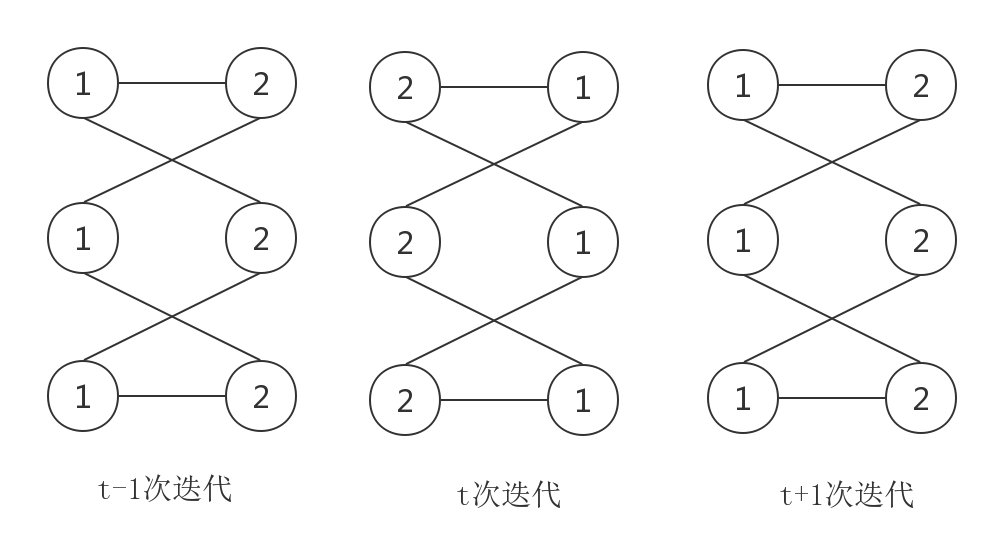
\includegraphics[width=0.75\textwidth]{figures/fig3-1}
 \caption{二分网络中的标签震荡现象}\label{fig:fig3-1}
\end{figure}

标签传播算法的设计方法简单,容易被人理解接受,算法的执行过程如算法
所示。

算法 :标签传播算法(LPA) 

输入:复杂网络 $G = (V, E)$,最大迭代次数 $maxRun$ 

输出:社区划分结果 

Step1:  初始化,为网络中的每个节点分配一个各不相同的标签,$c_i(0)=i$;令迭代次数$t=0$。

Step2:  标签传播迭代过程 

(a)如果迭代次数 $t > maxRun$,标签传播迭代过程结束,转 Step3;否则继续算法。 

(b)随机排列网络中的节点,并将节点顺序存放在向量 X 中。 

(c)对于每个节点$v_i\in X$,更新$c_i(t)=f(c_{i1}(t), c_{i2}(t),..., c_{im}(t))$表示在当次更新过程中节点$v_{i1}, ..., v_{im}$的邻接点中标签已经更新的节点集,表示在当次更新过程中节点的邻接点中标签还未更新的节点集。这里的函数$f(x)$将返回集合中出现频次最高的标签。如果返回不止一个标签,那么就在其中随机选择一个。 

(d)如果所有节点的标签都不再改变,那么标签传播迭代过程停止,转Step3;否则,令$t = t+1$转到步骤(a)继续执行。 

Step3:  社区划分,将拥有相同标签的节点划分到同一个社区中,不同标签的种类就表示网络中社区的个数。 
\usepackage{algorithm}  
\usepackage{algpseudocode}  
\usepackage{amsmath}  
\renewcommand{\algorithmicrequire}{\textbf{Input:}}  % Use Input in the format of Algorithm  
\renewcommand{\algorithmicensure}{\textbf{Output:}} % Use Output in the format of Algorithm  

\begin{algorithm}[h]  
  \caption{An example for format For \& While Loop in Algorithm}  
  \begin{algorithmic}[1]  
    \For{each $i\in [1,9]$}  
      \State initialize a tree $T_{i}$ with only a leaf (the root);  
      \State $T=T\cup T_{i};$  
    \EndFor  
    \ForAll {$c$ such that $c\in RecentMBatch(E_{n-1})$}  
      \label{code:TrainBase:getc}  
      \State $T=T\cup PosSample(c)$;  
      \label{code:TrainBase:pos}  
    \EndFor;  
    \For{$i=1$; $i<n$; $i++$ }  
      \State $//$ Your source here;  
    \EndFor  
    \For{$i=1$ to $n$}  
      \State $//$ Your source here;  
    \EndFor  
    \State $//$ Reusing recent base classifiers.  
    \label{code:recentStart}  
    \While {$(|E_n| \leq L_1 )and( D \neq \phi)$}  
      \State Selecting the most recent classifier $c_i$ from $D$;  
      \State $D=D-c_i$;  
      \State $E_n=E_n+c_i$;  
    \EndWhile  
    \label{code:recentEnd}  
  \end{algorithmic}  
\end{algorithm}  

LPA 算法每次迭代过程中更新节点的顺序随机确定,并且当多个标签在其邻接点中出现次数最多时,标签的更新也是随机的,因此每次执行标签传播算法都可能得到不同的社区划分结果。在众多的社区划分结果中,很难确定哪一个结果是最优的划分。所以解决标签传播算法的稳定性问题是非常有必要的,而且也是非常重要的。

\section{k-核分解方法}
在第二章第一小节社交网络的统计特性中,很多计算节点重要性的方法被提出,比如度、聚集系数和介数等。度和聚集系数仅能够衡量网络局部的信息;介数能够反映整个网络的全局信息,但是由于介数的计算需要计算网络中所有的最短路径,因此它的时间复杂度很高。Kitsak 等人[41]提出复杂网络中 k-核值高的节点对整个网络的信息传播是非常重要的,其传播能力强。

k-核分解方法是将复杂网络分解成若干子结构,子结构中的每个节点在该子
结构中的度最小为 k。为 k-核中的每个节点 i 分配一个 k-核值,用 Ks(i)表示,该
值表明节点 i 属于 k-核,但是不属于(k+1)-核。k-核值的大小反应了节点在网络中
的中心性地位,k-核分解方法经常被用于识别网络中的中心和边缘节点。

k-核分解方法的具体步骤如下:首先不断的将网络中度为 1 的节点及与这些
节点相连的边移除,直到剩余网络中不再有度为 1 的节点为止,并将移除的节点
划分为 1-核子集,并设置这些节点的 k-核值为 1;使用同样的方法,递归的移除
剩余网络中度为 2 或小于 2 的节点及连接这些节点的边,直到剩余网络中不再有
度为 2 或小于 2 的节点为止,创建 2-核子集;分解过程继续执行,直到网络中所
有的节点都被划分到相应的 k-核子集中。k-核值大(或小)的节点子集位于网络
的中心(或边缘)位置。通过 k-核分解方法能够得到网络的层次结构,该结构类
似于一个洋葱,反应了网络中节点完整的层次结构。k-核分解方法能够在线性时
间内执行完成,时间复杂度为 $O(|E|)$,其中|E|是网络中边的数量。

\section{异步标签传播策略}

异步标签传播策略能够避免标签震荡现象,并且相对同步标签更新策略需要
更少的迭代次数,因此这里采用异步标签更新方法。然而由于节点并不是同时更
新的,因此节点更新的顺序对社区发现结果的稳定性及社区质量有很大的影响;
除此之外,标签传播过程中的标签选择策略也存在不稳定因素,当返回多个标签
同时被最大个数邻接点拥有时,LPA 算法随机的选择其中的一个标签作为该节点
的新标签,这也造成了 LPA 算法的不稳定性。而 下一章节要提到的COPRA 中也同样存在这些不稳
定因素。

在简单网络上分析传统标签传播算法的社区发现过程,如图\ref{fig:fig3-2}所示。在
该网络中有两个社区,分别是${v_1,v_2,v_3}$和${v_4,v_5,v_6}$。节点上的数字表示该节点
的社区标签,初始的时候各个节点的社区标签各不相同,如图\ref{fig:fig3-2}(a)所示。假设
经过几次标签传播之后,节点拥有相同的标签“2”,而节点 $v_4$、$v_5$和 $v_6$
的标签仍然各不相同,如图\ref{fig:fig3-2}(b)所示。如果首先更新节点 $v_4$
的标签,由于它的所有邻接点的标签都各不相同,随机选择标签“2”作为节点 $v_4$
的新标签,
更新结果如图\ref{fig:fig3-2}(c)所示;然后更新节点 $v_6$
的标签为标签“2”,此时节点 $v_5$
的两个邻接点的标签都为“2”,它也更新为标签“2”。这样更新后所有的节点都划分
到了同一个社区中,这样的社区划分结果没有意义。相反,在更新节点 $v_4$
的标签时,如果随机选择的更新标签是标签“6”,如图 \ref{fig:fig3-2}(d)所示;紧接着更新节点$v_5$
的标签,根据标签计算公式得到节点 $v_5$
的新标签为标签“6”;此时节点 $v_6$的
两个邻接点的标签都为“6”,它的标签保持不变。通过这样的标签更新顺序和标
签选择方式,能够得到正确的社区划分结果。

\begin{figure}
  \centering
  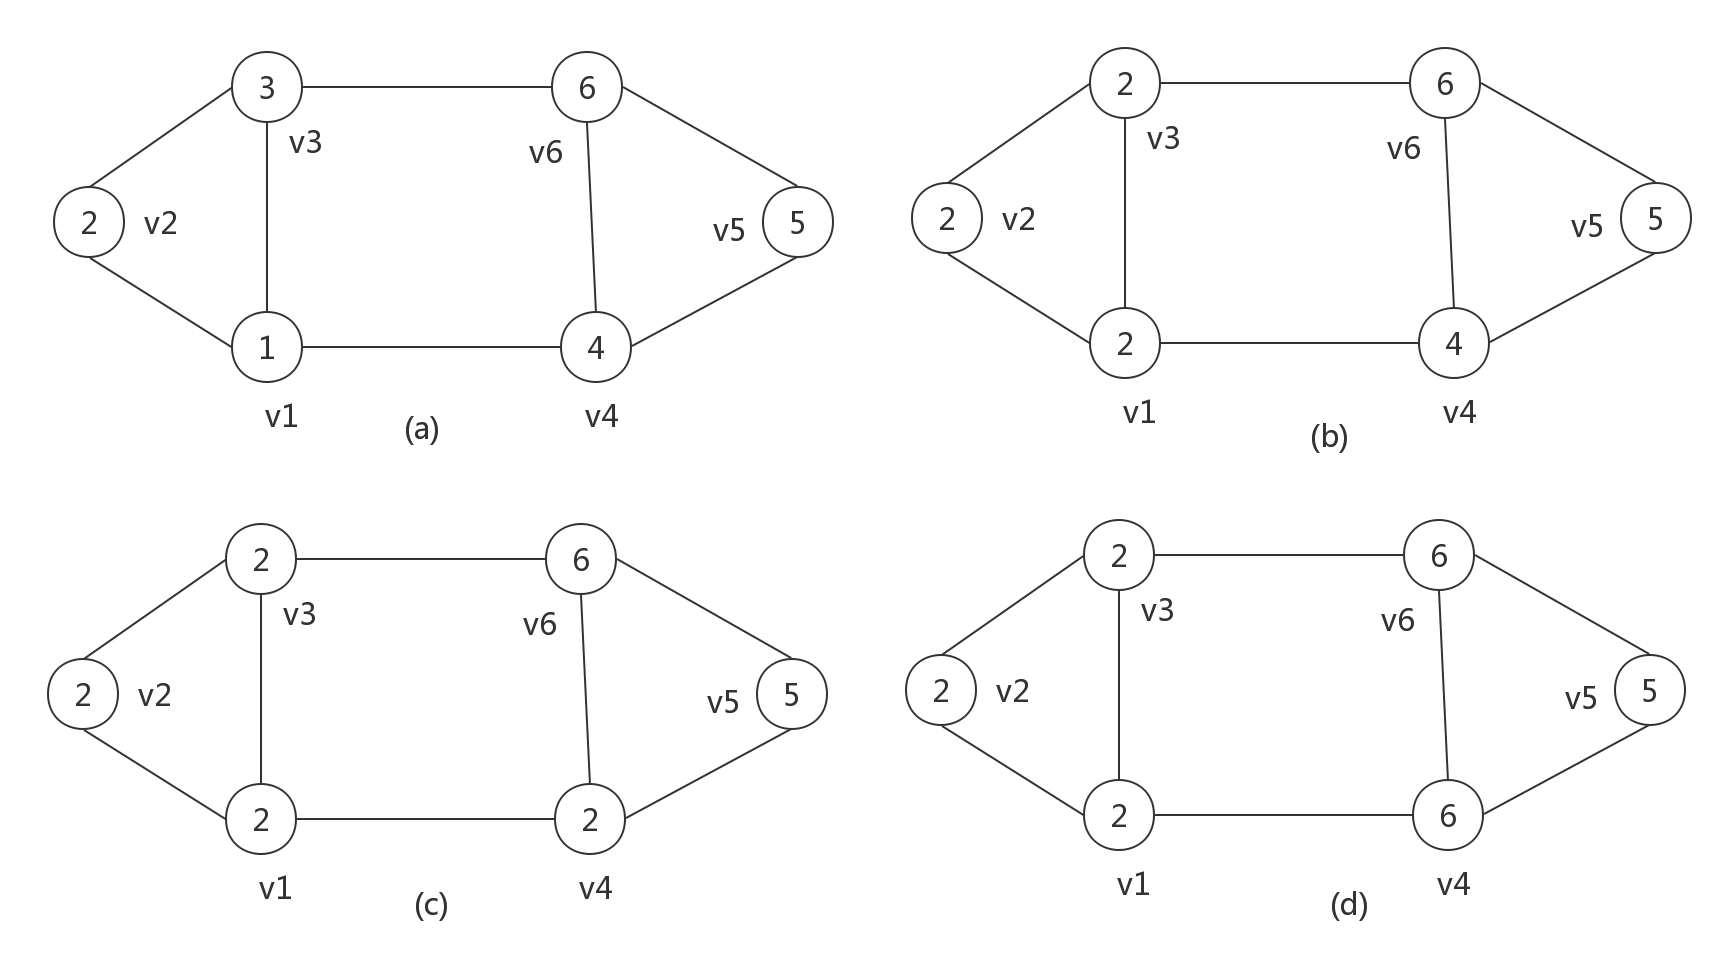
\includegraphics[width=0.75\textwidth]{figures/fig3-2}
  \caption{标签传播过程示意图}\label{fig:fig3-2}
\end{figure}

通过上面的分析,传统的异步标签传播算法对节点更新的顺序及标签选择方
法非常敏感,标签传播过程中的随机性不仅造成算法收敛速度的不同,甚至会影响最终的社区划分结果。因此,本章将提出一种改进的标签传播算法,克服传统
标签传播算法的不足。

\section{算法思想}
在CDABSLP算法中,仍采用异步更新策略来避免图\ref{fig:fig3-1}所示的标签震荡现象的出现。
但是,不确定的节点更新顺序导致算法的稳定性差,新算法中需要克服此问题。
在算法每次的更新过程中,先更新的节点的标签在整个标签传播过程中发挥的作
用比后更新的节点的标签的作用要大,这是因为后更新节点的新标签对已经更新
的节点的标签没有影响,最后一个更新的节点的新标签对其他所有节点的标签选
择都不会产生影响。因此,算法应该根据节点的重要性对节点进行排序,重要的
节点应该优先更新。 

k-核值大的节点表示它位于网络的核心位置,然而,在复杂网络中,有大量
节点拥有相同的 k-核值,因此,仅根据该指标对节点进行排序的效果并不好。通
常,在复杂网络中,一个节点如果和很多核心节点相连,那么该节点在网络中的
地位也是很重要的。受该思想的启发,本章提出一种同时考虑节点本身 k-核值和
其邻接点 k-核值共同影响的节点中心性衡量指标。节点 i 的影响值的计算如公式\ref{eqn:NI}

\begin{equation}
  \label{eqn:NI}
  NI(i)=Ks(i)+\alpha \times \sum_{j \in \Gamma _i} \frac{Ks(j)}{d_j}
\end{equation}

其中,$\alpha$是调节参数,取值范围从 0 到 1,用来调节邻接点对节点影响值的
作用大小。将公式\ref{eqn:jiedianyingxiangzhi}计算得到的节点影响值作为衡量节点重要性的指标,按节
点影响值降序对节点进行排序作为节点更新的顺序。固定节点更新顺序能够使算
法更加稳定。 

造成标签传播算法不稳定的另一个因素是标签选择的机制,当更新一个节点
的标签时,如果返回多个标签同时被最大个数的邻接点拥有时,传统的标签传播
算法会随机的从中选择一个标签赋给该节点,因此,算法迭代过程很难得到一个
稳定的收敛状态。为了提高算法的稳定性,当返回多个标签时,将节点影响值引
入到标签更新公式中,选择标签影响强度最大的标签赋给该节点。 

标签l对节点i的影响强度计算如公式\ref{eqn:LI}所示。

\begin{equation}
  \label{eqn:LI}
  NI(i,l)=\sum_{j \in \Gamma _i} \frac{NI(j)}{d_j}
\end{equation}

其中,$\Gamma _i$
表示节点i的邻接点中标签为l的节点集合。改进的节点标签更新公
式如公式\ref{eqn:ci}所示。

\begin{equation}
  \label{eqn:ci}
  c_i=\arg\max_{l \in lmax} LI(i,l)
\end{equation}

其中,$lmax $表示同时被最大个数邻接点拥有的标签集合。 
当传统标签传播算法的标签更新公式返回多个标签时,根据公式\ref{eqn:LI}计算这
些标签对该节点的影响强度,选择影响强度最大的标签赋给该节点。当标签影响
强度最大的标签仍有多个时,节点保留原有标签。 

\section{算法设计}
CDABSLP算法的主要步骤包括初始化、迭代标签传播和社区划分,图\ref{fig:fig3-3}为
CDABSLP算法的流程图。

\begin{figure}
  \centering
  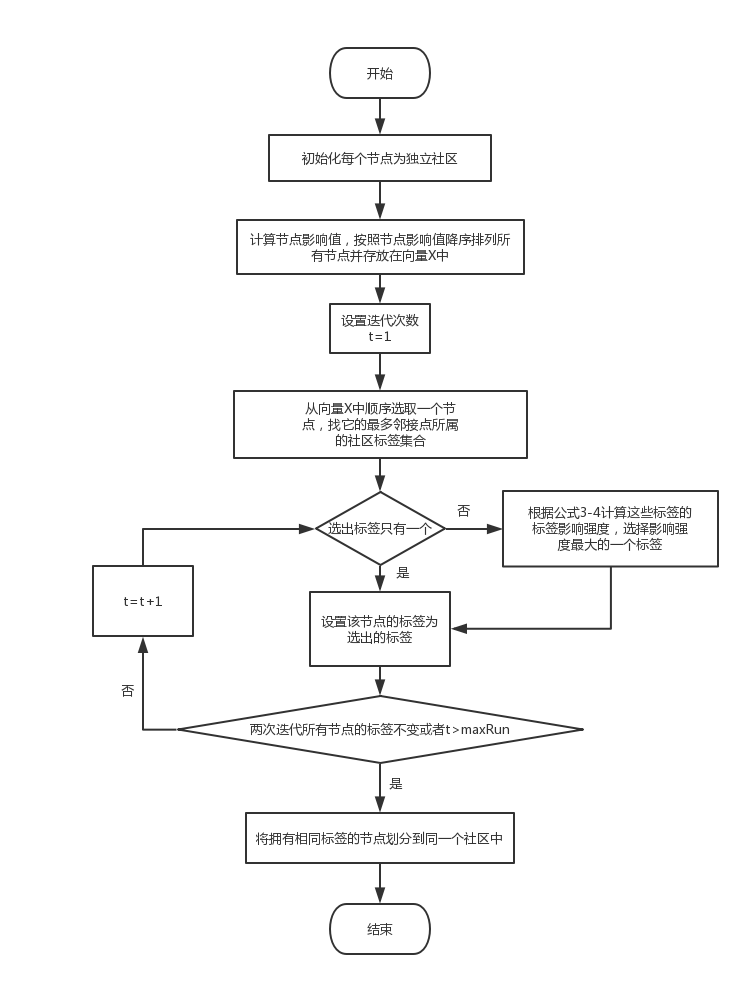
\includegraphics[width=1\textwidth]{figures/fig3-3}
  \caption{CDABSLP算法流程图}\label{fig:fig3-3}
 \end{figure}

通过一个简单的例子来展示 CDABSLP算法的执行过程,如图\ref{fig:fig3-4}所示,算法
中参数$\alpha =1$。图中每一个圆圈代表一个节点,节点间的连线代表节点间的边,
节点外的实数表示节点的影响值$ NI$。按节点影响值降序排列图中的节点$v_1-v_2-V_4-v_6-v_5$
(当节点影响值相同时,按节点的先后顺序排列),以该顺序作为
节点更新的顺序,标签更新过程如图\ref{fig:fig3-4}所示。

\begin{figure}
  \centering
  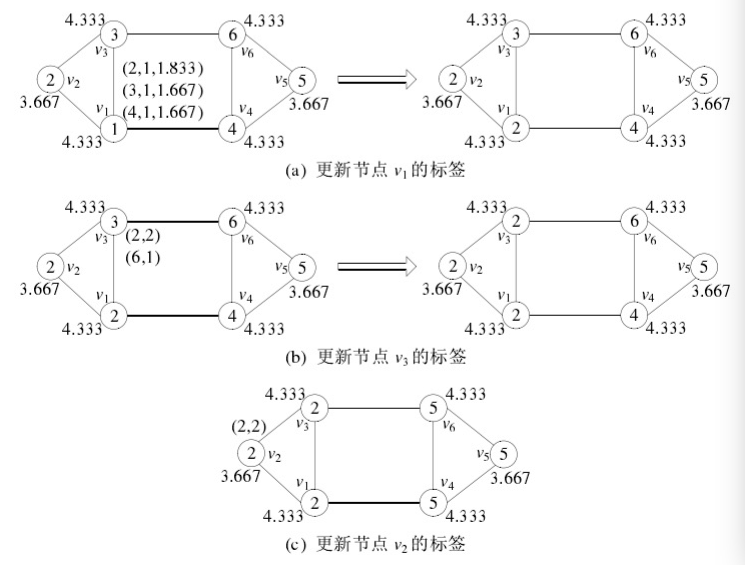
\includegraphics[width=0.75\textwidth]{figures/fig3-4}
  \caption{CDABSLP算法标签传播过程示意图}\label{fig:fig3-4}
 \end{figure}

 按照节点更新顺序,第一个更新节点$v_1$
的标签。首先为节点$v_1$计算一系列
的三元组$(l,|\Gamma _1^l|,LI(v_1,l))$,其中$ l $表示其邻接点中包含的标签,
$|\Gamma _1^l|$表示标签为
$l $的邻接点的个数,最后一项$LI(v_1,l)$表示标签对该节点的影响强度,该项是一个
可选项,当不能通过传统的标签选择策略得到一个确定的标签时,通过公式\ref{eqn:LI}
计算得到。如图\ref{fig:fig3-4}(a)所示,节点$ v_1
$有三个邻接点$ v_2$
、$v_3$和 $v_4$,并且它们的标签
各不相同,计算得到节点 $v_1$
对应的三元组集合为${(2, 1, 1.833), (3, 1, 1.667), (4, 1, 
1.667)}$。因此选择标签 2 作为节点 $v_1$
的新标签。 

接着更新节点 v3的标签。更新完节点 $v_1$的标签之后,如图\ref{fig:fig3-4}(a)右图所示,节点$ v_3$共有三个邻接点$ v_1$、$v_2$和$ v_6$,其中$ v_1$和$ v_2$的标签相同,均为标签 2,只有节点 $v_6$的标签不同。因此选择标签 2 作为节点 $v_3$的新标签,如图\ref{fig:fig3-4}(b)所示。接下来节点$ v_4$和$ v_6$标签的更新分别与节点$ v_1$和$ v_3$的情况相同,更新结果如图\ref{fig:fig3-4}(c)所示。

最后只有节点$ v_2$和$ v_5$没有更新,此时如图\ref{fig:fig3-4}(c)所示,节点 $v_2$和它的邻接点的标签都为标签 2,而节点 $v5$与它所有的邻接点的标签都为标签 5,因此节点$v_2$和$ v_5$的标签不需要改变。

通过执行 CDABSLP 算法,在该网络上仅需执行一次标签更新过程就得到了最
终稳定的社区划分结构,得到两个与真实情况一致的社区。由于算法的执行过程
中没有了随机因素的存在,因此算法的输出结果是确定的且优质的。 

\section{算法时间复杂度分析}
算法的时间复杂度分析如下,$|V|$表示网络中节点的个数,$|E|$表示网
络中边的数目。 

(1)为每个节点初始化标签所用时间复杂度为 $O(|V|)$; 

(2)计算网络中所有节点的影响值的时间复杂度为 $O(|E|)$; 

(3)按节点影响值降序排列网络中所有节点所用时间复杂度为
$O(|V|log(|V|))$;

(4)每次标签传播过程分为两部分: 传统的标签计算过程:$O(|E|)$; 当传统标签计算过程返回多个标签时,利用公式\ref{eqn:LI}重新计算节点标签的过程:$O(|E|)$; 

(5)将相同标签的节点划分到一个社区的时间复杂度为 $O(|V|)$。 

标签传播过程是不断迭代执行的,因此整个算法的时间复杂度为
$2O(|V|)+(2t+1)O(|E|)+O(|V|log(|V|))$,$t $表示迭代次数,一般通过比较少的迭
代次数就能得到最后的结果。 

\section{算法伪代码}